% This file was created with tikzplotlib v0.10.1.
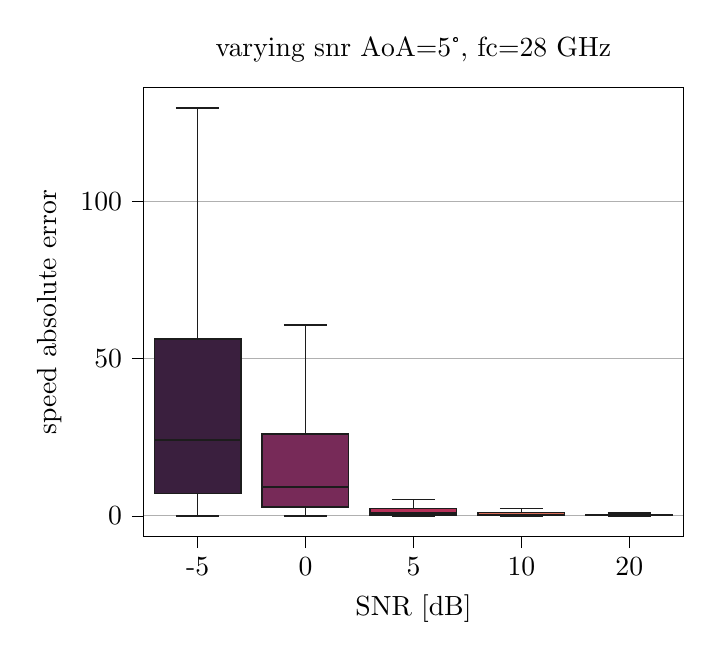
\begin{tikzpicture}

\definecolor{black28}{RGB}{28,28,28}
\definecolor{brown1814888}{RGB}{181,48,88}
\definecolor{burlywood231175145}{RGB}{231,175,145}
\definecolor{darkgray176}{RGB}{176,176,176}
\definecolor{darkslategray583162}{RGB}{58,31,62}
\definecolor{indianred21811088}{RGB}{218,110,88}
\definecolor{purple1194288}{RGB}{119,42,88}

\begin{axis}[
tick align=outside,
tick pos=left,
title={varying snr AoA=5°, fc=28 GHz},
x grid style={darkgray176},
xlabel={SNR [dB]},
xmin=-0.5, xmax=4.5,
xtick style={color=black},
xtick={0,1,2,3,4},
xticklabels={-5,0,5,10,20},
y grid style={darkgray176},
ylabel={speed absolute error},
ymajorgrids,
ymin=-6.48700526548055, ymax=136.227207599328,
ytick style={color=black}
]
\path [draw=black28, fill=darkslategray583162, semithick]
(axis cs:-0.4,7.13045972771867)
--(axis cs:0.4,7.13045972771867)
--(axis cs:0.4,56.2368271074319)
--(axis cs:-0.4,56.2368271074319)
--(axis cs:-0.4,7.13045972771867)
--cycle;
\path [draw=black28, fill=purple1194288, semithick]
(axis cs:0.6,2.78592668563491)
--(axis cs:1.4,2.78592668563491)
--(axis cs:1.4,25.9444282948389)
--(axis cs:0.6,25.9444282948389)
--(axis cs:0.6,2.78592668563491)
--cycle;
\path [draw=black28, fill=brown1814888, semithick]
(axis cs:1.6,0.324812420710113)
--(axis cs:2.4,0.324812420710113)
--(axis cs:2.4,2.29225267229384)
--(axis cs:1.6,2.29225267229384)
--(axis cs:1.6,0.324812420710113)
--cycle;
\path [draw=black28, fill=indianred21811088, semithick]
(axis cs:2.6,0.155448298662069)
--(axis cs:3.4,0.155448298662069)
--(axis cs:3.4,1.01836457981036)
--(axis cs:2.6,1.01836457981036)
--(axis cs:2.6,0.155448298662069)
--cycle;
\path [draw=black28, fill=burlywood231175145, semithick]
(axis cs:3.6,0.0684982538796586)
--(axis cs:4.4,0.0684982538796586)
--(axis cs:4.4,0.39260279812352)
--(axis cs:3.6,0.39260279812352)
--(axis cs:3.6,0.0684982538796586)
--cycle;
\addplot [semithick, black28]
table {%
0 7.13045972771867
0 0.000716539433831542
};
\addplot [semithick, black28]
table {%
0 56.2368271074319
0 129.740197923655
};
\addplot [semithick, black28]
table {%
-0.2 0.000716539433831542
0.2 0.000716539433831542
};
\addplot [semithick, black28]
table {%
-0.2 129.740197923655
0.2 129.740197923655
};
\addplot [semithick, black28]
table {%
1 2.78592668563491
1 0.00060882045378019
};
\addplot [semithick, black28]
table {%
1 25.9444282948389
1 60.6645388690484
};
\addplot [semithick, black28]
table {%
0.8 0.00060882045378019
1.2 0.00060882045378019
};
\addplot [semithick, black28]
table {%
0.8 60.6645388690484
1.2 60.6645388690484
};
\addplot [semithick, black28]
table {%
2 0.324812420710113
2 2.90530539377443e-05
};
\addplot [semithick, black28]
table {%
2 2.29225267229384
2 5.22887281566029
};
\addplot [semithick, black28]
table {%
1.8 2.90530539377443e-05
2.2 2.90530539377443e-05
};
\addplot [semithick, black28]
table {%
1.8 5.22887281566029
2.2 5.22887281566029
};
\addplot [semithick, black28]
table {%
3 0.155448298662069
3 1.35789885220561e-05
};
\addplot [semithick, black28]
table {%
3 1.01836457981036
3 2.31039606089282
};
\addplot [semithick, black28]
table {%
2.8 1.35789885220561e-05
3.2 1.35789885220561e-05
};
\addplot [semithick, black28]
table {%
2.8 2.31039606089282
3.2 2.31039606089282
};
\addplot [semithick, black28]
table {%
4 0.0684982538796586
4 4.41019254981967e-06
};
\addplot [semithick, black28]
table {%
4 0.39260279812352
4 0.878363895507487
};
\addplot [semithick, black28]
table {%
3.8 4.41019254981967e-06
4.2 4.41019254981967e-06
};
\addplot [semithick, black28]
table {%
3.8 0.878363895507487
4.2 0.878363895507487
};
\addplot [semithick, black28]
table {%
-0.4 24.201944488185
0.4 24.201944488185
};
\addplot [semithick, black28]
table {%
0.6 9.19319344795474
1.4 9.19319344795474
};
\addplot [semithick, black28]
table {%
1.6 0.963734229266757
2.4 0.963734229266757
};
\addplot [semithick, black28]
table {%
2.6 0.441415752835742
3.4 0.441415752835742
};
\addplot [semithick, black28]
table {%
3.6 0.173593959884562
4.4 0.173593959884562
};
\end{axis}

\end{tikzpicture}
